\documentclass[border=0pt]{standalone}
\usepackage{mathptmx}
\usepackage{amssymb}
\usepackage[scaled=0.92]{helvet}
\renewcommand{\familydefault}{\sfdefault}
\usepackage[dvipsnames]{xcolor}
\usepackage{tikz}
\usetikzlibrary{positioning,fit,backgrounds,arrows.meta,calc,shapes.geometric,shadows}
\definecolor{caindigo}{HTML}{4F46E5}
\definecolor{cagreen}{HTML}{059669}
\definecolor{caorange}{HTML}{EA580C}
\definecolor{caslate}{HTML}{475569}
\definecolor{cared}{HTML}{DC2626}
\definecolor{caviolet}{HTML}{8B5CF6}
\definecolor{cabgindigo}{HTML}{EEF2FF}
\definecolor{cabggreen}{HTML}{ECFDF5}
\definecolor{cabgorange}{HTML}{FFF7ED}
\definecolor{cabgslate}{HTML}{F8FAFC}
\definecolor{cabgred}{HTML}{FEF2F2}
\definecolor{cadark}{HTML}{312E81}
\begin{document}
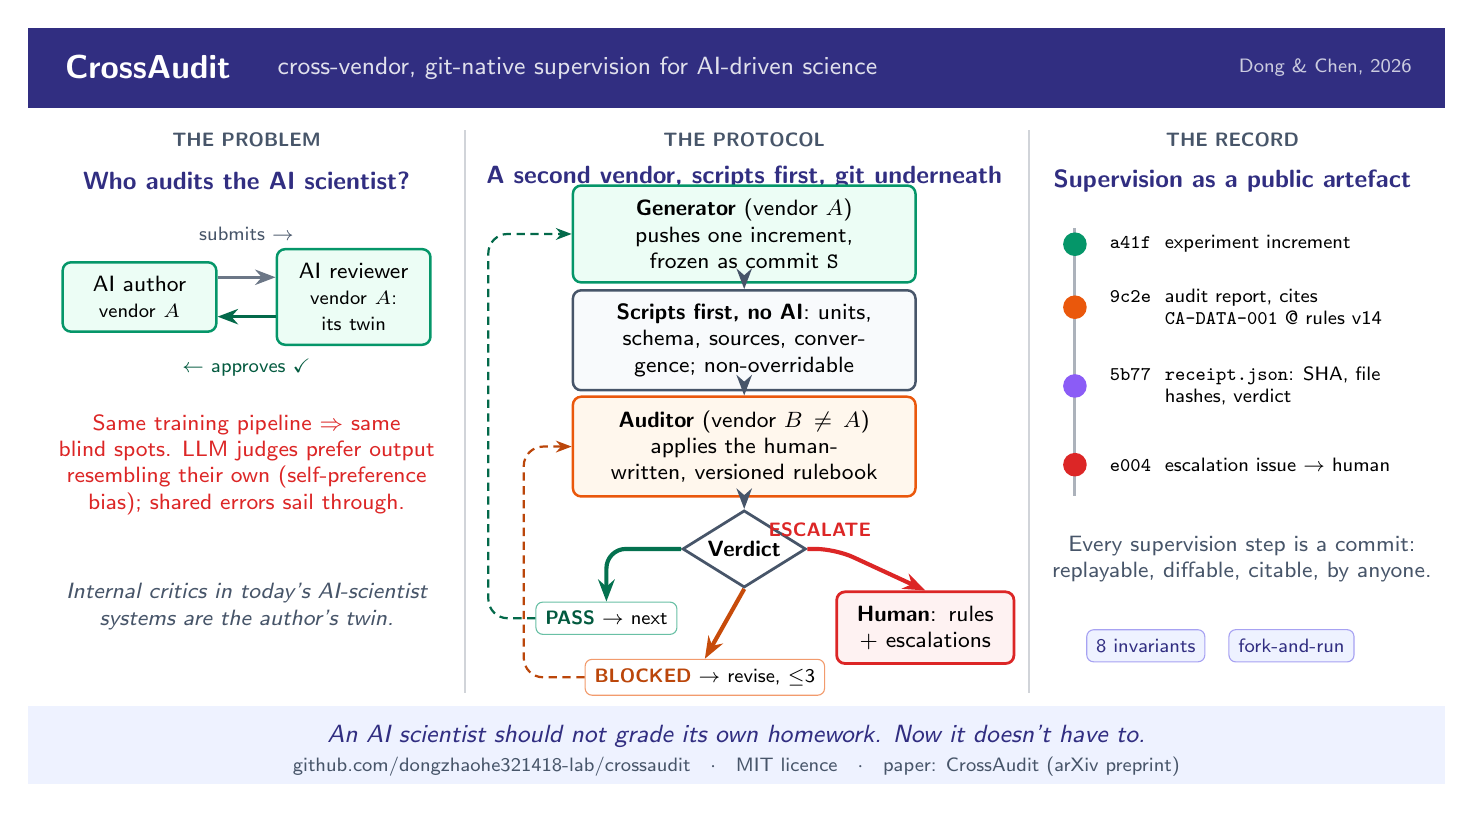
\begin{tikzpicture}[x=1cm, y=1cm,
  font=\footnotesize,
  box/.style={draw, rounded corners=3pt, align=center, inner sep=5pt, line width=0.9pt},
  hdr/.style={font=\scriptsize\bfseries, text=caslate},
  flow/.style={-{Stealth[length=2.6mm]}, line width=1.2pt, draw=caslate},
  fate/.style={-{Stealth[length=2.8mm]}, line width=1.5pt, rounded corners=7pt},
  ret/.style={-{Stealth[length=2mm]}, line width=0.8pt, densely dashed, rounded corners=7pt},
  chip/.style={rounded corners=2.5pt, inner sep=3.4pt, font=\scriptsize, fill=white}
]
\path (0,0) rectangle (18,-9.6);
% ---------- banner ----------
\fill[cadark] (0,0) rectangle (18,-1.02);
\node[anchor=west, text=white, font=\large\bfseries] at (0.35,-0.50) {CrossAudit};
\node[anchor=west, text=white!85!cadark, font=\small] at (3.05,-0.51) {cross-vendor, git-native supervision for AI-driven science};
\node[anchor=east, text=white!75!cadark, font=\scriptsize] at (17.7,-0.51) {Dong \& Chen, 2026};
% ---------- panel dividers ----------
\draw[caslate!25, line width=0.6pt] (5.55,-1.30) -- (5.55,-8.45);
\draw[caslate!25, line width=0.6pt] (12.72,-1.30) -- (12.72,-8.45);
% ================= PANEL 1: the problem =================
\node[hdr] at (2.78,-1.42) {THE PROBLEM};
\node[align=center, font=\small\bfseries, text=cadark] at (2.78,-1.95) {Who audits the AI scientist?};
\node[align=center, font=\scriptsize, text=caslate] at (2.78,-2.62) {submits $\rightarrow$};
\node[box, draw=cagreen, fill=cabggreen, text width=16mm] (a1) at (1.42,-3.42) {AI author\\ \scriptsize vendor $A$};
\node[box, draw=cagreen, fill=cabggreen, text width=16mm] (a2) at (4.14,-3.42) {AI reviewer\\ \scriptsize vendor $A$: its twin};
\draw[flow, draw=caslate!80] ([yshift=2.5mm]a1.east) -- ([yshift=2.5mm]a2.west);
\draw[flow, draw=cagreen!70!black] ([yshift=-2.5mm]a2.west) -- ([yshift=-2.5mm]a1.east);
\node[align=center, font=\scriptsize, text=cagreen!60!black] at (2.78,-4.32) {$\leftarrow$ approves $\checkmark$};
\node[align=center, text=cared, font=\footnotesize] at (2.78,-5.55) {Same training pipeline $\Rightarrow$ same\\ blind spots. LLM judges prefer output\\ resembling their own (self-preference\\ bias); shared errors sail through.};
\node[align=center, font=\footnotesize\itshape, text=caslate] at (2.78,-7.35) {Internal critics in today's AI-scientist\\ systems are the author's twin.};
% ================= PANEL 2: the protocol =================
\node[hdr] at (9.10,-1.42) {THE PROTOCOL};
\node[align=center, font=\small\bfseries, text=cadark] at (9.10,-1.90) {A second vendor, scripts first, git underneath};
\node[box, draw=cagreen, fill=cabggreen, text width=40mm] (g) at (9.10,-2.62) {\textbf{Generator} (vendor $A$) pushes one increment, frozen as commit \texttt{S}};
\node[box, draw=caslate, fill=cabgslate, text width=40mm] (d) at (9.10,-3.97) {\textbf{Scripts first, no AI}: units, schema, sources, convergence; non-overridable};
\node[box, draw=caorange, fill=cabgorange, text width=40mm] (b) at (9.10,-5.32) {\textbf{Auditor} (vendor $B \neq A$) applies the human-written, versioned rulebook};
\node[draw=caslate, fill=white, diamond, aspect=1.6, inner sep=1.8pt, line width=1pt] (v) at (9.10,-6.62) {\footnotesize\textbf{Verdict}};
\draw[flow] (g) -- (d); \draw[flow] (d) -- (b); \draw[flow] (b) -- (v);
% fates: three branches out of the diamond
\node[chip, draw=cagreen!60] (cp) at (7.35,-7.50) {\textcolor{cagreen!60!black}{\textbf{PASS}} $\to$ next};
\node[chip, draw=caorange!60] (cb) at (8.60,-8.25) {\textcolor{caorange!80!black}{\textbf{BLOCKED}} $\to$ revise, $\leq$3};
\node[box, draw=cared, fill=cabgred, text width=19mm, line width=1pt] (h) at (11.40,-7.62) {\textbf{Human}: rules $+$ escalations};
\draw[fate, draw=cagreen!75!black] (v.west) -| (cp.north);
\draw[fate, draw=caorange!85!black] (v.south) -- (cb.north);
\draw[fate, draw=cared] (v.east) -- node[sloped, above=0.2mm, font=\scriptsize\bfseries, text=cared, pos=0.45]{ESCALATE} (h.north west |- v.east) -- (h.north);
% thin dashed returns: the loop closes
\draw[ret, draw=cagreen!70!black] (cp.west) -- (5.85,-7.50) -- (5.85,-2.62) -- (g.west);
\draw[ret, draw=caorange!80!black] (cb.west) -- (6.30,-8.25) -- (6.30,-5.32) -- (b.west);
% ================= PANEL 3: the record =================
\node[hdr] at (15.30,-1.42) {THE RECORD};
\node[align=center, font=\small\bfseries, text=cadark] at (15.30,-1.95) {Supervision as a public artefact};
\draw[caslate!45, line width=1.1pt] (13.30,-2.55) -- (13.30,-5.95);
\foreach \y/\c/\t in {
  -2.75/cagreen/{\texttt{a41f}~ experiment increment},
  -3.55/caorange/{\texttt{9c2e}~ audit report, cites\\ \hphantom{\texttt{9c2e}~} \texttt{CA-DATA-001} @ rules v14},
  -4.55/caviolet/{\texttt{5b77}~ \texttt{receipt.json}: SHA, file\\ \hphantom{\texttt{5b77}~} hashes, verdict},
  -5.55/cared/{\texttt{e004}~ escalation issue $\to$ human}}{
  \fill[\c] (13.30,\y) circle (1.5mm);
  \node[anchor=west, align=left, font=\scriptsize] at (13.62,\y) {\t};}
\node[align=center, font=\footnotesize, text=caslate] at (15.42,-6.75) {Every supervision step is a commit:\\ replayable, diffable, citable, by anyone.};
\node[chip, draw=caindigo!50, fill=cabgindigo, text=cadark] at (14.20,-7.85) {8 invariants};
\node[chip, draw=caindigo!50, fill=cabgindigo, text=cadark] at (16.05,-7.85) {fork-and-run};
% ---------- footer ----------
\fill[cabgindigo] (0,-8.62) rectangle (18,-9.6);
\node[align=center, font=\small\itshape, text=cadark] at (9,-9.00) {An AI scientist should not grade its own homework. Now it doesn't have to.};
\node[align=center, font=\scriptsize, text=caslate] at (9,-9.38) {github.com/dongzhaohe321418-lab/crossaudit \; $\cdot$ \; MIT licence \; $\cdot$ \; paper: CrossAudit (arXiv preprint)};
\end{tikzpicture}
\end{document}
